\documentclass[11pt, a4paper]{article}

\usepackage[utf8]{inputenc}
\usepackage[T1]{fontenc}
\usepackage{amsmath}
\usepackage{amssymb}
\usepackage{graphicx}
\usepackage{geometry}
\usepackage{fancyhdr}
\usepackage{enumitem}
\usepackage{array}
\usepackage{eso-pic}
\usepackage{esvect}
\usepackage{tikz}
\usetikzlibrary{arrows.meta,calc}
\usepackage{siunitx}
\DeclareSIUnit{\litre}{l}
\sisetup{
    locale = DE,
    inter-unit-product = \cdot,
    per-mode = symbol-or-fraction
}

\geometry{a4paper, top=2.5cm, bottom=2.5cm, left=2.5cm, right=2.5cm}

\makeatletter
\def\input@path{{./}{../../}}
\makeatother
\graphicspath{{Bilder/Allgemein/}{../../Bilder/Allgemein/}}

\input{defs}

\pagestyle{fancy}
\fancyhf{}
\cfoot{\thepage}

\begin{document}
% Command to add the logo to the top left of the first page
\AddToShipoutPictureBG*{%
  \AtPageUpperLeft{%
    \hspace{2.0cm}% Move logo to the right from the page edge
    \raisebox{-5.cm}{% Move logo down from the page edge
            
\includegraphics[width=4cm]{LogoFHCampus.png}% The logo file
    }%
  }%
}

\begin{center}
    {\Large \textbf{Physikalische Grundlagen}} \\[1em]
    {\large Kurztest 3: Dynamik (Kräfte)} \\[1em]
    {\large Studiengang: Clinical Engineering}
\end{center}

\vspace{1cm}

\noindent
\vspace{1cm}
\noindent
\begin{tabular}{ll}
    \textbf{Kürzel:} & \underline{\hspace{8cm}} \\[0.5cm]
    \textbf{Gruppe: } & \LARGE\textbf{A}  \\[0.3cm]
\end{tabular}

\begin{itemize}[label={$\circ$}]
    \item Sie haben 25 min Zeit.
    \item Sie dürfen einen Taschenrechner verwenden.
    \item Geben Sie klare und verständliche Antworten!
    \item Schreiben Sie leserlich!
    \item Sie dürfen $g = \SI{10}{\meter\per\second\squared}$ verwenden.
\end{itemize}

Viel Erfolg!

\vspace{2cm}

\begin{flushright}
    \renewcommand{\arraystretch}{1.23}
    \begin{tabular}{l p{2.3cm}}
        \hline
        \noalign{\vskip 0.15cm}
        \textbf{\Large{Punkte:}} & \textbf{\Large{/10 }} \\
        \noalign{\vskip 0.1cm}
        \hline
    \end{tabular}
\end{flushright}

\newpage

\begin{enumerate}[label=\textbf{\arabic*.},itemsep=0.45cm]
    \vspace{0cm}

    \item (1,5 P) - \textbf{Newtonschen Axiome:} \\
    Geben Sie die drei Newtonschen Axiome an und erläutern Sie kurz, was jedes Axiom besagt.
    \begin{itemize}
        \item 1. Newtonsches Axiom: \\[0.03cm]
        \item 2. Newtonsches Axiom: \\[0.03cm]
        \item 3. Newtonsches Axiom:
    \end{itemize}

    \item (1,5 P) - \textbf{Kraft aus Beschleunigung:} \\
    Es wirken die folgenden drei Kräfte auf einen Körper der Masse \(m = 2\, \text{kg}\): 
    \begin{equation*}
        \vec{F}_1 = \begin{pmatrix} 3 \\ 0 \\ -1 \end{pmatrix} \, \text{N}, \quad \vec{F}_2 = \begin{pmatrix} 0 \\ 4 \\ 2 \end{pmatrix} \, \text{N}, \quad \vec{F}_3 = \begin{pmatrix} -5 \\ 2 \\ 7 \end{pmatrix} \, \text{N}
    \end{equation*}
    Berechne die resultierende Kraft \(\vec{F}_{\text{res}}\) und die Beschleunigung \(\vec{a}\) des Körpers.

    \item (2 P) - \textbf{Reibung auf der schiefen Ebene:} \\
    Ein Körper der Masse \(m = 5\, \text{kg}\) liegt unter dem Einfluss der Schwerkraft auf einer schiefen Ebene, die einen Winkel von \(\alpha = 30^\circ\) zur Horizontalen bildet. Der Haftreibungskoeffizient beträgt $\mu_H = \SI{0.4}{}$. Wird der Körper auf der schiefen Ebene gehalten oder beginnt er zu rutschen? Zeichnen Sie die Gravitationskraft \(F_G\), die Normalkraft \(F_N\) und die Hangabtriebskraft \(F_A\) in die Skizze ein. Berechnen Sie nun die Hangabtriebskraft \(F_A\) und die maximale Haftreibungskraft \(F_{R,h,\text{max}}\). 
    \begin{center}
        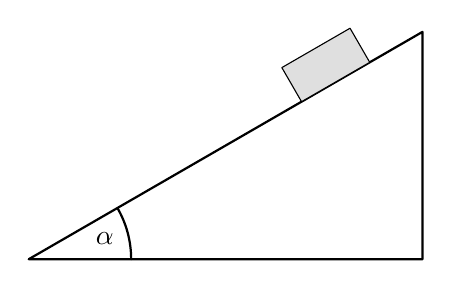
\begin{tikzpicture}[scale=1.0, >=Latex, line cap=round, line join=round]
            \coordinate (A) at (0,0);
            \coordinate (B) at (5,0);
            \coordinate (C) at (5,2.88675);
            \coordinate (P) at ($(A)+(30:4)$);
            \coordinate (M) at ($(P)+(30:0.5)+(120:0.25)$);
            \coordinate (Gend) at ($(M)+(0,-2)$);
            \coordinate (Aend) at ($(M)+(210:1.)$);

            \draw[thick] (A) -- (B) -- (C) -- (A);

            \draw[fill=gray!25, rotate around={30:(P)}] ($(P)$) rectangle ($(P)+(1,0.5)$);

            \draw[thick] ($(A)+(1.3,0)$) arc[start angle=0,end angle=30,radius=1.3];
            \node at ($(A)+(15:1.0)$) {$\alpha$};

        \end{tikzpicture}
        \end{center}

    \item (1 P) - \textbf{Federkraft:} \\
    Eine Feder hat eine Federkonstante von \(k = \SI{150}{\newton\per\meter}\). Welche Kraft wirkt auf die Feder (achten Sie auf das Vorzeichen), wenn sie um $\Delta x = \SI{0.2}{\meter}$ bzw. $\Delta x = \SI{-1}{\meter}$ gedehnt wird? 

    \item (1 P) - \textbf{Feder-Masse-System:} \\
    Unter dem Einfluss der Schwerkraft hängt eine Masse von \SI{2}{\kilogram} an einer Feder mit \(k = \SI{200}{\newton\per\meter}\). Das System ist im Gleichgewicht. Wie groß ist die Dehnung der Feder?

    \item (1,5 P) - \textbf{Geschwindigkeit des Körpers im Hookeschen Gesetz} \\
    Sie möchten eine Formel für die Geschwindigkeit eines Körpers mit Masse $m$ bestimmen, der an einer Feder mit Federkonstante $k$ hängt. Zeigen Sie, dass das unweigerlich auf die Gleichung 
    \begin{equation*}
        m \cdot v \cdot \mathrm{d}v = -k \cdot x \cdot \mathrm{d}x
    \end{equation*}
    hinausläuft, wobei $x$ die Auslenkung der Feder von der Ruhelage ist. \\
    \textit{Tipp: }Ersetzen Sie im Hookeschen Gesetz die Kraft $F$ mithilfe des 2. Newtonschen Axioms. Anschließend verwenden Sie die Kettenregel $\cfrac{da}{dc} = \cfrac{da}{db} \, \cfrac{db}{dc}$. 

    \item (1,5 P) - \textbf{Integration der Geschwindigkeit:} \\
    In der vorherigen Aufgabe haben Sie die Gleichung 
    \begin{equation*}
        m \cdot v \cdot \mathrm{d}v = -k \cdot x \cdot \mathrm{d}x
    \end{equation*}
    hergeleitet. Integrieren Sie diese Gleichung, um eine Formel für die Geschwindigkeit \(v\) in Abhängigkeit von der Auslenkung \(x\) zu erhalten. Nehmen Sie an, dass die Geschwindigkeit \(v = 0\) ist, wenn die Auslenkung \(x = A\) (die maximale Auslenkung) beträgt.
    \begin{equation*}
        v = 
    \end{equation*}
\end{enumerate}

\end{document}